% Template for PLoS
% Version 3.1 February 2015
%
% To compile to pdf, run:
% latex plos.template
% bibtex plos.template
% latex plos.template
% latex plos.template
% dvipdf plos.template
%
% % % % % % % % % % % % % % % % % % % % % %
%
% -- IMPORTANT NOTE
%
% This template contains comments intended 
% to minimize problems and delays during our production 
% process. Please follow the template instructions
% whenever possible.
%
% % % % % % % % % % % % % % % % % % % % % % % 
%
% Once your paper is accepted for publication, 
% PLEASE REMOVE ALL TRACKED CHANGES in this file and leave only
% the final text of your manuscript.
%
% There are no restrictions on package use within the LaTeX files except that 
% no packages listed in the template may be deleted.
%
% Please do not include colors or graphics in the text.
%
% Please do not create a heading level below \subsection. For 3rd level headings, use \paragraph{}.
%
% % % % % % % % % % % % % % % % % % % % % % %
%
% -- FIGURES AND TABLES
%
% Please include tables/figure captions directly after the paragraph where they are first cited in the text.
%
% DO NOT INCLUDE GRAPHICS IN YOUR MANUSCRIPT
% - Figures should be uploaded separately from your manuscript file. 
% - Figures generated using LaTeX should be extracted and removed from the PDF before submission. 
% - Figures containing multiple panels/subfigures must be combined into one image file before submission.
% For figure citations, please use "Fig." instead of "Figure".
% See http://www.plosone.org/static/figureGuidelines for PLOS figure guidelines.
%
% Tables should be cell-based and may not contain:
% - tabs/spacing/line breaks within cells to alter layout or alignment
% - vertically-merged cells (no tabular environments within tabular environments, do not use \multirow)
% - colors, shading, or graphic objects
% See http://www.plosone.org/static/figureGuidelines#tables for table guidelines.
%
% For tables that exceed the width of the text column, use the adjustwidth environment as illustrated in the example table in text below.
%
% % % % % % % % % % % % % % % % % % % % % % % %
%
% -- EQUATIONS, MATH SYMBOLS, SUBSCRIPTS, AND SUPERSCRIPTS
%
% IMPORTANT
% Below are a few tips to help format your equations and other special characters according to our specifications. For more tips to help reduce the possibility of formatting errors during conversion, please see our LaTeX guidelines at http://www.plosone.org/static/latexGuidelines
%
% Please be sure to include all portions of an equation in the math environment.
%
% Do not include text that is not math in the math environment. For example, CO2 will be CO\textsubscript{2}.
%
% Please add line breaks to long display equations when possible in order to fit size of the column. 
%
% For inline equations, please do not include punctuation (commas, etc) within the math environment unless this is part of the equation.
%
% % % % % % % % % % % % % % % % % % % % % % % % 
%
% Please contact latex@plos.org with any questions.
%
% % % % % % % % % % % % % % % % % % % % % % % %

\documentclass[10pt,letterpaper]{article}
\usepackage[top=0.85in,left=2.75in,footskip=0.75in]{geometry}

% Use adjustwidth environment to exceed column width (see example table in text)
\usepackage{changepage}

% Use Unicode characters when possible
\usepackage[utf8]{inputenc}

% textcomp package and marvosym package for additional characters
\usepackage{textcomp,marvosym}

% fixltx2e package for \textsubscript
\usepackage{fixltx2e}

% amsmath and amssymb packages, useful for mathematical formulas and symbols
\usepackage{amsmath,amssymb}

% cite package, to clean up citations in the main text. Do not remove.
\usepackage{cite}

% Use nameref to cite supporting information files (see Supporting Information section for more info)
\usepackage{nameref,hyperref}

% line numbers
\usepackage[right]{lineno}

% ligatures disabled
\usepackage{microtype}
\DisableLigatures[f]{encoding = *, family = * }

% rotating package for sideways tables
\usepackage{rotating}

% Remove comment for double spacing
%\usepackage{setspace} 
%\doublespacing

% Text layout
\raggedright
\setlength{\parindent}{0.5cm}
\textwidth 5.25in 
\textheight 8.75in

% Bold the 'Figure #' in the caption and separate it from the title/caption with a period
% Captions will be left justified
\usepackage[aboveskip=1pt,labelfont=bf,labelsep=period,justification=raggedright,singlelinecheck=off]{caption}

% Use the PLoS provided BiBTeX style
\bibliographystyle{plos2015}

% Remove brackets from numbering in List of References
\makeatletter
\renewcommand{\@biblabel}[1]{\quad#1.}
\makeatother

% Leave date blank
\date{}

% Header and Footer with logo
\usepackage{lastpage,fancyhdr,graphicx}
\usepackage{epstopdf}
\pagestyle{myheadings}
\pagestyle{fancy}
\fancyhf{}
\lhead{
\includegraphics[width=2.0in]{PLOS-submission.eps}}
\rfoot{\thepage/\pageref{LastPage}}
\renewcommand{\footrule}{\hrule height 2pt \vspace{2mm}}
\fancyheadoffset[L]{2.25in}
\fancyfootoffset[L]{2.25in}
\lfoot{\sf PLOS}

%% Include all macros below

\newcommand{\lorem}{{\bf LOREM}}
\newcommand{\ipsum}{{\bf IPSUM}}

%% END MACROS SECTION


\begin{document}
\vspace*{0.35in}

% Title must be 250 characters or less.
% Please capitalize all terms in the title except conjunctions, prepositions, and articles.
\begin{flushleft}
{\Large
\textbf\newline{VCFLIB: an ensemble of methods for variant manipulation and population genetics }
}
\newline
% Insert author names, affiliations and corresponding author email (do not include titles, positions, or degrees).
\\

Erik Garrison\textsuperscript{2,\Yinyang},
Mark Yandell\textsuperscript{3,4},
Mike Shapiro\textsuperscript{5,3},
Gabor Marth\textsuperscript{3,4},
Richard Durbin\textsuperscript{2},
Evan E. Eichler\textsuperscript{1},
The VCFLIB Consortium\textsuperscript{\textpilcrow},
Zev N. Kronenberg\textsuperscript{1,\Yinyang, *},
\\
\bigskip
\bf{1} Department of Genome Sciences, University of Washington, Seattle, WA, USA
\\
\bf{2} Wellcome Trust Sanger Institute, Cambridge, UK
\\
\bf{3} Department of Human Genetics, University of Utah, Salt Lake City, UT, USA
\\
\bf{4} Ustar Center for Genetic Discovery, University of Utah, Salt Lake City, UT, USA

\bf{5} Department of Biology, University of Utah, Salt Lake City, UT, USA
\\
\bigskip

% Insert additional author notes using the symbols described below. Insert symbol callouts after author names as necessary.
% 
% Remove or comment out the author notes below if they aren't used.
%
% Primary Equal Contribution Note
\Yinyang These authors contributed equally to this work.

% Additional Equal Contribution Note
% Also use this double-dagger symbol for special authorship notes, such as senior authorship.
\ddag These authors also contributed equally to this work.

% Current address notes
\textcurrency a Insert current address of first author with an address update
% \textcurrency b Insert current address of second author with an address update
% \textcurrency c Insert current address of third author with an address update

% Deceased author note
%\dag Deceased

% Group/Consortium Author Note
\textpilcrow Membership list can be found in the Acknowledgments section.

% Use the asterisk to denote corresponding authorship and provide email address in note below.
* zevk@uw.edu

\end{flushleft}
% Please keep the abstract below 300 words
\section*{Abstract}




\linenumbers

\section*{Introduction}

Genetic variation is commonly represented in the Variant Call Format (VCF)\cite{vcftools}.  VCF files are flat-text, human-readable, and provide a flexible way to annotate genetic information.  When compressed, VCF records can be indexed and queried by genomic position\cite{tabix}. One or more genomes can be represented in the VCF genotype fields, which is important for population-level sequencing experiments. For these reasons, VCF has been widely adopted for large-scale genetic studies including the The 1000 Genomes Project \cite{1kg}, ExAC \cite{exac}, GoNL \cite{gonl}.

To the uninitiated, the VCF format, while easy to comprehend can be difficult to parse and manipulate. There is an ongoing need for methods that can facilitate rapid genetic analyses of VCF data.  VCFLIB, VCFTools\cite{vcftools}, GATK,  and BioConductor are software packages that are commonly used, each fulfilling a niche. 

This article is a milepost for VCFLIB development and showcases the population-level genetic analyses that can be done with the toolkit. In the Design and implementation section, we described the three attributes of VCFLIB: a C++ library, an ensemble of programs for modifying VCF files, and a toolkit for population genetics (The Genotype Phenotype Association Toolkit: GPAT). In the results section we apply VCFLIB to the 1000 Genomes Project data to quantify patterns of genetic variation within and between populations.  Lastly, we briefly discuss our goals for future VCFLIB development.


%\begin{equation}\label{eq:schemeP} 
%D_{coll} = \frac{D_f+\frac{[S]^2}{K_D S_T} D_S} {1+\frac{[S]^2}{K_D S_T}}, 
%D_{sm} = \frac{D_f+ \frac{[S]}{K_D} D_S}{1+\frac{[S]}{K_D}},
%\end{equation}

% You may title this section "Methods" or "Models". 
% "Models" is not a valid title for PLoS ONE authors. However, PLoS ONE
% authors may use "Analysis" 
\section*{Design and Implementation}



\subsection*{The VCFLIB library}

\subsection*{VCFLIB programs}



\subsection*{The Genotype Phenotype Association Toolkit (GPAT)}

The genotype-phenotype association toolkit was originally designed to map the genetic basis of phenotypic variation, but it has grown into a fully functional population genetic toolkit.  The GPAT association test, p F$_{ST}$ , has been successfully used to identify genetic variants associated with phenotypic variation in domestic pigeons
 \cite{color},  and \textit{Tetrahymena}\cite{tet}.  GPAT has also been used for basic summary statistics, like heterzoygosity and allele frequency, in human\cite{iron} and pigeon\cite{pigeon} populations.




\paragraph*{ F$_{ST}$  methods} \mbox{} \\

The Weir and Cockerham estimator of F$_{ST}$ is implemented in GPAT`s ``wcF$_{ST}$ " \cite{fst}.  The method filters mulit-allelic VCF records and sites where less than five individuals are present in the target or background population. Values of F$_{ST}$ will range from slightly negative to one; negative values are treated as zero in downstream GPAT analyses. 

An independent bayesian estimator of F$_{ST}$ is provided in GPAT \cite{bfst}.  The method, implemented in ``bF$_{ST}$ ", has free parameters for the allele frequencies in the target and background populations, and F$_{ST}$.  The posterior distribution of F$_{ST}$ is generated by 50,000 Markov chain Monte Carlo iterations.  This method generates credible intervals around each F$_{ST}$ value.  Because this method requires MCMC it is computationally expensive and should only be used on small regions.

Smoothing F$_{ST}$  values in a window is an intuitive way to deal with the high F$_{ST}$ variance between physically close genetic variants.  GPAT's ``smoother" program provides a way to average  F$_{ST}$  values across a user defined window and step size.  It is good practice to explore different window sizes because of the goldilocks principle; Windows that are too large dilute local signals while small windows suffer from noise.

To circumnavigate the issues with soothing we have introduced an algorithm that locates the beginning and end of a region with high  F$_{ST}$.  The tool, ``segment F$_{ST}$", scans the output of ``wc F$_{ST}$ " measuring the number of  F$_{ST}$  values that are above a user-defined threshold in a window of ten F$_{ST}$ values.  If the low to high  F$_{ST}$  ratio is above two the window is recursively extended.  This heuristic, unlike a sliding window, does not suffer from the goldilocks principle.  However, it is dependent on the user defined F$_{ST}$ threshold.  For both smoothing and segmenting it is important to visualize the results to make sure that the window size and segmentation threshold are appropriate for the data.

The empirical significance of the smoothed windows or segmented  F$_{ST}$ can be quantified using the permutation tool, ``permuteSmooth".  The program takes the raw F$_{ST}$ values and the smoothed or segmented F$_{ST}$  data.  The windows or segments are shuffled across the genome to regions with the same number of  F$_{ST}$  values.  The empirical probability is calculated as the number of random trial where the average  F$_{ST}$  was higher than the observed window/segment.  ``permuteSmooth" is threaded to reduce the runtime of the permutation test.  To rank the output we recommend sorting by the imperial p-value followed by the size of the window or segment.

\paragraph*{$\Delta$ allele frequency (AF) and association tests} \mbox{} \\

The difference in allele frequencies ($\Delta$) between two phenotypically distinct groups can be used to idnetify genetic variants associated with a trait of interest.  A likelihood test for $\Delta$ AF is implemented in ``pF$_{ST}$ " for both pooled and genotypic data Eq~(\ref{eq:pfst}).   In Eq~(\ref{eq:pfst }), \textit{B} represented the binomial distribution parameterized by the number of trials \textit{n}, the number of successes \textit{k} and the probability of success, \textit{p}.  The \textit{D} statistic is chi-squared distributed with one degree of freedom.

\begin{equation}\label{eq:pfst} 
D=-2* ln (\frac{ B(n_c,k_c,p_c) }{ B(n_t,k_t,p_t)*B(n_b,k_b,p_b)  })
\end{equation}

In pF$_{ST}$, \textit{n} corresponds to the number of callable alleles, \textit{k} is the number on non-reference alleles, and \textit{p} is the bounded allele frequency (0.00001-0.99999).  The subscripts denotes the group membership for the target (\textit{t}), background (\textit{b}) and both combined (\textit{c}).  If genotype likelihoods are provided, pF$_{ST}$  weights each allele proportionally to the genotype likelihood, rather than the direct count.   For pooled datasets, with more than one biological replicate in the target and background, the model substitutes the binomial distribution for the beta.  The methods of moments used to estimate $\alpha$, and $\beta$, the two parameters of the beta distribution.  The likelihood ratio-test implemented in pF$_{ST}$ is widely discussed \cite{kim,heng}, but few practical implementations exist.  

There are several limitations of pFst.  First, pFst does not account for population structure.  If the target and background populations are not well matched many genetic variants will be highly scored.  pFst was not designed for quantitive traits.  However, if the target and background represent the extremes of the phenotypic range pFst can be used.  Tools like PLINK \cite{plink}, EMMA\cite{emma}, and TASSLE\cite{tassel} provide more robust statistical models for associations testing.

\paragraph*{Haplotype methods (for phased variants) }\mbox{} \\

GPAT provides several methods for quantifying haplotype structure at a locus.  The extended haplotype homozygosity (EHH) score measures the haplotypic diversity; a value of zero means all haplotypes are unique and a value of one means all haplotypes are identical. The ``sequenceDiversity" program quantifies EHH (Eq~[\ref{eq:EHH}]) across a fixed number of positions (user defined). In Eq~\ref{eq:EHH} \textit{n} is the number of chromosomes (2x the number of genotypes), \textit{i} is the index for each unique haplotype in a fixed window and \textit{x\textsubscript{i}} is the number of \textit{i} haplotypes.  


\begin{equation}\label{eq:EHH} 
EHH=\frac{\sum_{i} \binom{x_i}{2}}{\binom{n}{2}}
\end{equation}

\begin{equation}\label{eq:EHHC} 
EHH_c=\frac{\sum_{ic} \binom{x_{ic}}{2}}{\binom{n_c}{2}}
\end{equation}

The integrated haplotype score (iHS) measures the relative decay of \textit{EHH\textsubscript{c}} (Eq~[\ref{eq:EHHC}]) between the alternative and reference core haplotypes,  Eq~(\ref{eq:iHS})\cite{voight}.  At a single variant position (core haplotype), \textit{EHH\textsubscript{c}} equals one and \textit{n\textsubscript{c}} is the number of reference or alternative alleles.  The trapezoid rule is used to integrate  \textit{EHH\textsubscript{c}} with respect to genetic distance.  GPAT's implementation of iHS uses PLINK formatted genetic maps\cite{plink}.  If no map file is provided, a fixed genetic distance of 0.001 is used.  GPAT also provides a tool ( ``normalize-iHS") to normalize iHS binned by allele frequency of the variants.  Comparison of GPAT iHS and other tools can be seen in Fig S1\cite{selscan}\cite{voight}.

\begin{equation}\label{eq:iHS} 
iHS = ln(\frac{\int \textrm{\textit{EHH}}_{c(alt)}}{ \int \textrm{EHH}_{c(ref)} } )
\end{equation}


% Results and Discussion can be combined.
\section*{Results}

As a demonstration of the power and flexibility of VCFLIB we performed within and between population genome-wide selection scans on the Phase III One Thousand Genomes Project data\cite{1kg}.  We measured population stratification between Northern Europeans (CEU), Southern Han Chinese (CHB), and Yoruba (YRI) using Weir and Cockerham's  F$_{ST}$. To detect within-population selection we applied the integrated haplotype score (iHS).  These analyses serve as a good control for VCFLIB methodology as many studies have perviously identified genes under selection in CEU, CHB, and YRI \cite{pickrell, sabeti, mathieson, weir}.  The VCLIB workflows used in the selection studies are shown in Fig. 1E and Fig. 2A.

\begin{figure}[h]

%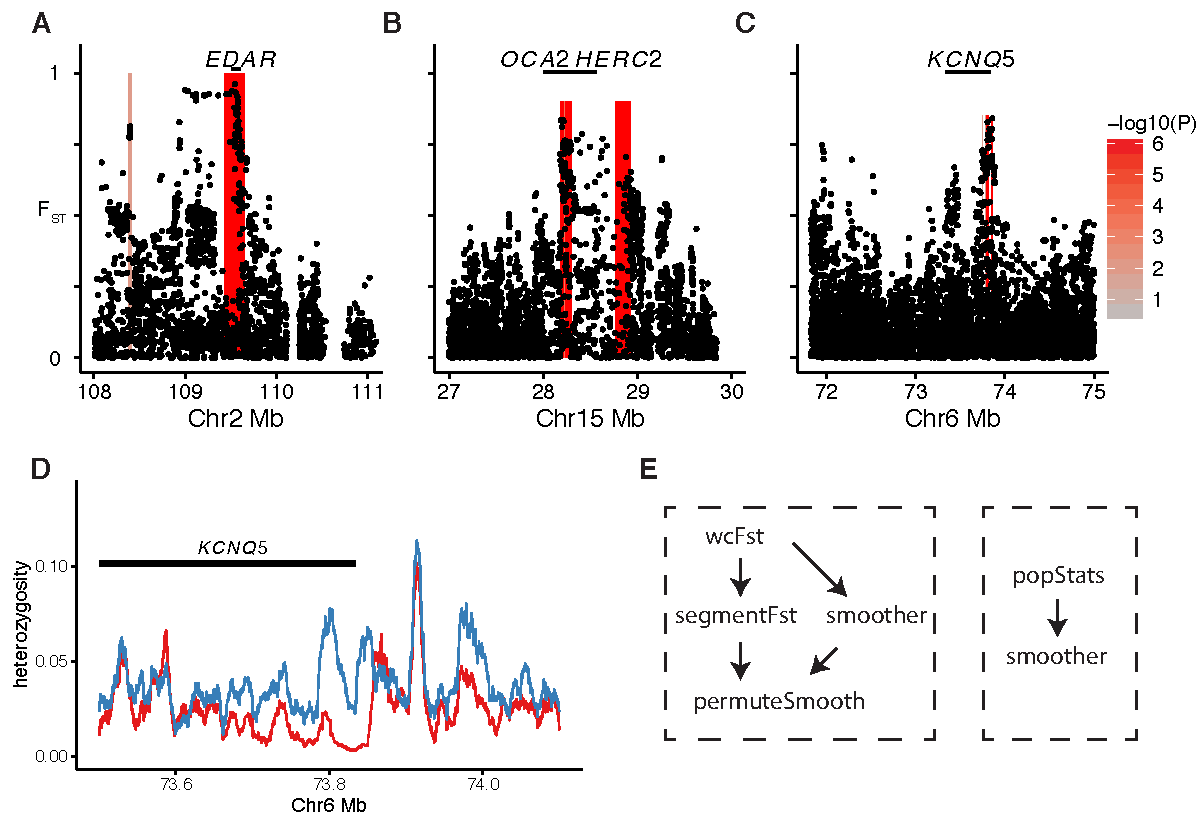
\includegraphics[width=0.95\textwidth]{Fig1}
\caption{{\bf Using VCFLIB to find population stratified loci in the One Thousand Genomes Project data.} The  F$_{ST}$  scatter plots (A-C) show genomic position on the x-axis and Weir and Cockerham's  F$_{ST}$  on the y-axis.  The vertical bands delineate regions of high  F$_{ST}$  defined by segment F$_{ST}$ .  The color of the bands denotes the empirical significance of the region compared to the rest of the genome determined with permuteSmooth.  A: \textit{EDAR} is an outlier in the CEU-CHB comparison because \textit{EDAR} is under selection in CHB.  B: \textit{OCA2} and \textit{HERC2} are outliers in the CEU-CHB comparison because they are under selection in CEU.  The segmentation of the region is broken by segmental duplications between ~28-29 Mb.  C: \textit{KCNQ5} is an outlier in the CEU-YRI comparison.  D:  KCNQ5 shows decreased heterozygosity at it's 3' (~73.9Mb) end in CEU (red) compared with YRI (blue).  E: The  F$_{ST}$  workflow used to identify candidate loci and the heterozygosity workflow used in the \textit{KCNQ5} example.}
\label{fig1}
\end{figure}

\begin{figure}[h]

%\includegraphics[width=0.95\textwidth]{Fig2}
\caption{{\bf Using VCFLIB to identify patterns of haplotype diversity consistent with natural selection.} A: The GPAT 
workflows used for the haplotype analysis. B: Genome-wide iHS Manhattan plot for Norther Europeans (CEU).  The x-axis is an index and the y-axis is the average absolute iHS within a 100Kbs sliding window.  The repeating color palette delineates chromosomes.  Several iHS peaks are annotated with the closest gene or a dash if there was not a gene nearby. The window that overlaps lactase has the highest genome-wide average iHS.  C: The lactase haplotypes present in CEU and YRI.  Each row is a single haplotype and each column is a position where there is a non-reference allele (red).  Fewer unique haplotypes can be seen in CEU compared to YRI.   The zoomed region denotes where the haplotype plots are located in relation to lactase. D:  The Extended Haplotype Homozygosity (EHH) decay for rs3754686(A/G).  Chromosomal position is shown on the x-axis and EHH for the derived (orange) and ancestral allele (green) is shown on the y-axis.}
\label{fig2}
\end{figure}

\subsection*{Detecting population stratified loci with VCFLIB}

The three population pair-wise F$_{ST}$ comparisons resulted in over 30 million data points. To identify genomic regions with exceptional  F$_{ST}$ values, we applied ``segmentFst" with a threshold of 0.6.   There were 3,790, 1,826, and 665 regions with high F$_{ST}$  values for the CHB-YRI, CEU-YRI and CEU-CHB comparisons, respectively.  These regions overlapped 254 genes in CEU-CHB, 578 genes in CEU-YRI, and 1,047 genes in CHB-YRI.   To assess the empirical significance of the high  F$_{ST}$ regions, we ran a permutation test for one million iterations.  At a stringent p-value cutoff (p $<$ 1e-5) there were 175 genes for CEU-CHB, 213 genes for CEU-YRI, and 407 genes for the CHB-YRI datasets (Table S1).   

Classic examples of loci that are known targets of natural selection were present amongst our top hits. When comparing CHB to CEU, Ectodysplasin A receptor (\textit{EDAR}) was in a segment with the lowest tier of p-values (p $<$ 1e-6), shown in Fig. 1A. In a mouse model a single amino substitution in \textit{EDAR} affects hair thickness, the number of eccrine sweat glands and increases mammary glad branching \cite{edar}. In another example, the genes \textit{OCA2} and \textit{HERC} were top hits in the CEU CHB comparison (Fig. 1B).  Variants in the \textit{OCA2} promoter, within a \textit{HERC2} intron, affect the expression of \textit{OCA2}, a major locus for eye color\cite{oca2}.  

To test if there was pathway enrichment for the stratified loci, we ran DAVID with the highest classification stringency and constrained the analysis to segmented loci with and empirical p-value less than 1e-5\cite{david}. In all three gene lists there were no terms within functional clusters that reached significance after Benjamini-Hochberg correction.  While pathway enrichment was not fruitful, we noticed a recurrence of genes expressed in the brain.  For example, \textit{KCNQ5} was highly differentiated between CEU and YRI, shown in Fig. 1C.  Lowered heterozygosity in CEU was observed toward the end of \textit{KCNQ5}  (Fig. 1D).  Dominant-negative \textit{KCNQ5} alleles, in mice, have been shown to affect neuronal action potential in the CA3 hippocampus\cite{kcnq5}.  In another example, \textit{POGZ}, a gene that is has been associated with intellectual disability and autism spectrum disorders was found in the CEU-CHB comparison, see Fig. S2.  While the patterns of F$_{ST}$ around many of these loci are consistent with selection, much more work is required to prove a significant correlation.

\subsection*{Detecting recent selection using VCFLIB}

For the iHS analyses we smoothed the data, counting the fraction of absolute iHS values above 2.5 in a 100Kbs sliding window.  Windows with less than 20\% high iHS values or fewer than 50 observations were filtered out. There were 313,049 windows before filtering for the three datasets and 3,616 windows after filtering.  A total of 2,083 genes intersect these windows (560 YRI, 921 CEU, and 1043 CHB).  The unfiltered results can found in Table S2. 

Within the CEU population the lactase genes (\textit{LCT}) had the highest iHS score, see Fig. 2B.  The HLA locus, \textit{NRG3}, \textit{KIAA0556} and \textit{ALG12} also stood out as candidates of selection.  To visualize the haplotypic structure around \textit{LCT} we used the ``plotHaps" program.  Increased haplotype sharing within CEU can be seen over \textit{LCT} compared to YRI, Fig. 2C.  The highest EHH values were upstream of LCT within the \textit{MCM6} gene, Fig. 2D.  The top hits in YRI were regions with genes involved in host-pathogen interaction.  The Chemokine receptors \textit{CCR1} and \textit{CCR3} were in a window with an average iHS score of 2.79 and over 50\% of iHS scores in the window were above 2.5. Two windows on different chromosomes  (Chr1 and Chr3) contained The Poliovirus receptor-Related 3 and 4.  Genes within CHB outlier regions included the nucleotide-sugar transporter \textit{SLC35D1}, Cut-like Homeobox \textit{CUX1}, \textit{TRIM44} and \textit{RBFOX2}.

\subsection*{Conclusions}

In this paper we have described the functionality of the VCFLIB for variant manipulation and population genetic applications.  The selection analyses discussed here show how GPAT tools, built upon VCFLIB, can be used to rapidly describe patterns of genetic variation within and between populations directly from a VCF file.  By recapitulating the findings of prior selection scans we demonstrate that our new automated methods for outlier discovery (``segmentFst", ``smoother", and ``permuteSmooth") are reliable.  While we focused on selection analyses in this paper, the entire VCFLIB toolkit has much more to offer. VCF comparison, format conversion, filtering and subsetting, annotation, variant representation, genotype manipulation are all functions contained within the VCFLIB repository.  We hope continued community involvement will allow VCFLIB to expand to match the need for reliable open source software for high throughput sequencing experiments. 

\section*{Availability and Future Directions}

VCFLIB is publicly available at (\url{https://github.com/vcflib/vcflib}{VCFLIB}).  We support community involvement on github, gitter and Biostars.org.  Areas of continued development include extending documentation, unit testing,  support for new VCF specifications, and additional population genetic metrics.  We would like add selection tests based on the allele frequency spectrum like Tajima's D and Achaz's Y\cite{achaz}.  Additionally we hope to make our selection tests results available in a public genome browser like the 1000 Genomes Selection Browse \cite{pybus}.



\section*{Supporting Information}

% Include only the SI item label in the subsection heading. Use the \nameref{label} command to cite SI items in the text.
\subsection*{S1 Snakemake}
\label{S1_snakemake}
{\bf  F$_{ST}$  analyses.}  The snakemake file for the CEU-CHB  F$_{ST}$  analysis.  

\subsection*{S2 Snakemake}
\label{S2_snakemake}
{\bf iHS analyses.}  An archive of the snakemake file, the config file and region file used to run the CEU iHS analyses.

\subsection*{S1 Fig}
\label{S1_Fig}
{\bf Comparison of iHS methods.}  Scatter plots comparing VCFLIB's implementation of iHS to SELSCAN or Prichard's iHS. The iHS data are from a two megabase window around \textit{LCT} in CEU.

\subsection*{S1 Table}
\label{S1_Table}
{\bf Regions with high  F$_{ST}$  values.} The CEU-YRI, CEU-CHB, and CHB-YRI regions are in three different excel sheets.  The region in GRCh37 coordinates, the average  F$_{ST}$  values, and the empirical significance are listed as column headers.

\section*{Acknowledgments}

We would like to thank the countless number of people who have contributed suggestions, created bug reports, and modified the VCFLIB codebase.  

\subsection*{The VCFLIB Consortium}

EJ Osborne\textsuperscript{1},
Brett Kennedy\textsuperscript{1},
Daniel Ence\textsuperscript{1},
Travis Collier\textsuperscript{1},
EJ Osborne\textsuperscript{1},
...
\nolinenumbers

%\section*{References}
% Either type in your references using
% \begin{thebibliography}{}
% \bibitem{}
% Text
% \end{thebibliography}
%
% OR
%
% Compile your BiBTeX database using our plos2015.bst
% style file and paste the contents of your .bbl file
% here.
% 
\begin{thebibliography}{10}
\bibitem{1kg}
Sudmant, Peter H., et al. ``An integrated map of structural variation in 2,504 human genomes." Nature 526.7571 (2015): 75-81.

\bibitem{gonl}
Genome of the Netherlands Consortium. ``Whole-genome sequence variation, population structure and demographic history of the Dutch population." Nature Genetics 46.8 (2014): 818-825.

\bibitem{vcftools}
Danecek, Petr, et al. ``The variant call format and VCFtools." Bioinformatics 27.15 (2011): 2156-2158.

\bibitem{exac}
Exome Aggregation Consortium (ExAC), Cambridge, MA, http://exac.broadinstitute.org/, Feb 2016.

\bibitem{selscan}
Szpiech, Zachary A., and Ryan D. Hernandez. ``selscan: an efficient multithreaded program to perform EHH-based scans for positive selection." Molecular biology and evolution 31.10 (2014): 2824-2827.

\bibitem{voight}
Voight, Benjamin F., et al. ``A map of recent positive selection in the human genome." PLoS Biol 4.3 (2006): e72.

\bibitem{pigeon}
Shapiro, Michael D., et al. ``Genomic diversity and evolution of the head crest in the rock pigeon." Science 339.6123 (2013): 1063-1067.

\bibitem{tet}
Galati, Domenico F., et al. ``DisAp-dependent striated fiber elongation is required to organize ciliary arrays." The Journal of cell biology 207.6 (2014): 705-715.

\bibitem{bfst}
Holsinger, Kent E., Paul O. Lewis, and Dipak K. Dey. ``A Bayesian approach to inferring population structure from dominant markers." Molecular Ecology 11.7 (2002): 1157-1164.

\bibitem{fst}
Weir, Bruce S., and C. Clark Cockerham. ``Estimating F-statistics for the analysis of population structure." evolution (1984): 1358-1370.

\bibitem{kim}
Kim, Su Yeon, et al. ``Design of association studies with pooled or un?pooled next?generation sequencing data." Genetic epidemiology 34.5 (2010): 479-491.

\bibitem{heng}
Li, Heng. ``A statistical framework for SNP calling, mutation discovery, association mapping and population genetical parameter estimation from sequencing data." Bioinformatics 27.21 (2011): 2987-2993.

\bibitem{color}
Domyan, Eric T., et al. "Epistatic and combinatorial effects of pigmentary gene mutations in the domestic pigeon." Current Biology 24.4 (2014): 459-464.

\bibitem{iron}
Barber, Matthew F., and Nels C. Elde. "Escape from bacterial iron piracy through rapid evolution of transferrin." Science 346.6215 (2014): 1362-1366.

\bibitem{tabix}
Li, Heng. ``Tabix: fast retrieval of sequence features from generic TAB-delimited files." Bioinformatics 27.5 (2011): 718-719.

\bibitem{edar}
Kamberov, Yana G., et al. ``Modeling recent human evolution in mice by expression of a selected EDAR variant." Cell 152.4 (2013): 691-702.

\bibitem{oca2}
Eiberg, Hans, et al. ``Blue eye color in humans may be caused by a perfectly associated founder mutation in a regulatory element located within the HERC2 gene inhibiting OCA2 expression." Human genetics 123.2 (2008): 177-187.

\bibitem{knq5}
Tzingounis, Anastassios V., et al. ``The KCNQ5 potassium channel mediates a component of the afterhyperpolarization current in mouse hippocampus." Proceedings of the National Academy of Sciences 107.22 (2010): 10232-10237.

\bibitem{emma}
Zhou, Xiang, and Matthew Stephens. ``Genome-wide efficient mixed-model analysis for association studies." Nature genetics 44.7 (2012): 821-824.

\bibitem{plink}
Purcell, Shaun, et al. ``PLINK: a tool set for whole-genome association and population-based linkage analyses." The American Journal of Human Genetics 81.3 (2007): 559-575.

\bibitem{tassel}
Bradbury, Peter J., et al. ``TASSEL: software for association mapping of complex traits in diverse samples." Bioinformatics 23.19 (2007): 2633-2635.

\bibitem{pickrell}
Pickrell, Joseph K., et al. ``Signals of recent positive selection in a worldwide sample of human populations." Genome research 19.5 (2009): 826-837.

\bibitem{sabeti}
Sabeti, Pardis C., et al. ``Genome-wide detection and characterization of positive selection in human populations." Nature 449.7164 (2007): 913-918.

\bibitem{mathieson}
Mathieson, Iain, et al. ``Genome-wide patterns of selection in 230 ancient Eurasians." Nature 528.7583 (2015): 499-503.
\bibitem
Huang DW, Sherman BT, Lempicki RA. ``Systematic and integrative analysis of large gene lists using DAVID Bioinformatics Resources". Nature Protoc. 2009;4(1):44-57.

\bibitem{weir}
Weir, Bruce S., et al. ``Measures of human population structure show heterogeneity among genomic regions." Genome research 15.11 (2005): 1468-1476.

\bibitem{achaz}
Achaz, Guillaume. ``Frequency spectrum neutrality tests: one for all and all for one." Genetics 183.1 (2009): 249-258.

\bibitem{pybus}
Pybus, Marc, et al. ``1000 Genomes Selection Browser 1.0: a genome browser dedicated to signatures of natural selection in modern humans." Nucleic acids research (2013): gkt1188.


\end{thebibliography}



\end{document}

